% Plantilla TFG LaTeX LSI por:
%   Agustín Borrego <borrego@us.es>
%   Inma Hernández <inmahernandez@us.es>
% Su uso y modificación es libre.

% ̀¡Recuerda hacer copias de seguridad frecuentes durante la redacción del trabajo!
% Puedes descargar todo el código fuente del proyecto en zip en Menú > (Descargar) Fuente

\documentclass[12pt]{report}

% Paquetes LaTeX y estilos globales
\input{etc/pkgs}
\input{etc/style}

%%%%%%%%%%%%%%%%%%%%%%%%%%%%%%%%%%%%%%%%%%%%%%%%%%%%%%%%%%%%%%%%%%%%%%%%%%%%%%%%%%%%%

% Variables para la portada
\setTitle{Smart Grids: Control de Redes Eléctricas con Inteligencia Artificial}
\setAuthor{Daniel López Ramos} % Si hay más de un autor, separarlos con \\
\setDegree{Grado en Ingeniería Informática - Ingeniería del Software} % Cambiar si es necesario
\setSupervisor{David Gutiérrez Avilés \\ Manuel Barragán Villarejo} % Si hay más de un tutor, separarlos con \\
\setDepartment{Lenguajes y Sistemas Informáticos}
\setMonth{junio} % Dejar sólo el mes de la convocatoria en que se presenta el trabajo
\setYear{2025/26} % Por ejemplo, 2022/23

%%%%%%%%%%%%%%%%%%%%%%%%%%%%%%%%%%%%%%%%%%%%%%%%%%%%%%%%%%%%%%%%%%%%%%%%%%%%%%%%%%%%%

% Dedicatoria del trabajo
% Si no se desea incluir, comentar o borrar la línea siguiente para eliminar la página de dedicatoria
\setDedication{A la memoria de mi abuela, por su ejemplo de perseverancia. Mi abuela hobbit, que concentraba en metro y medio el amor de mil vidas.}

%%%%%%%%%%%%%%%%%%%%%%%%%%%%%%%%%%%%%%%%%%%%%%%%%%%%%%%%%%%%%%%%%%%%%%%%%%%%%%%%%%%%%

% Comienzo del documento
\begin{document}

    % Portada y secciones no numeradas
    \input{sections/00_portada}
    \input{sections/00_agradecimientos}
    \chapter*{Resumen}
La creciente integración de fuentes de energía renovable, la generación distribuida y la adopción masiva de tecnologías emergentes están introduciendo un nivel de complejidad radical en el sistema eléctrico. Este nuevo paradigma limita la viabilidad operativa de los métodos matemáticos de optimización tradicionales debido a sus altos costes computacionales y problemas de escalabilidad en tiempo real.

El objetivo principal consiste es desarrollar y evaluar modelos predictivos basados en técnicas de aprendizaje supervisado capaces de estimar, de forma ágil y precisa, los valores de referencia óptimos para el control de la red. Concretamente, la investigación se centra en predecir la inyección estratégica de potencia reactiva por parte de los generadores distribuidos, con el fin de minimizar las pérdidas de energía del sistema y mantener los perfiles de tensión dentro de límites seguros.

Para ello, se construye un \textit{pipeline} analítico que procesa datos temporales y aplica validación cruzada secuencial para garantizar la integridad de los resultados. La investigación analiza arquitecturas de ensamblaje como \textit{Random Forest} y \textit{XGBoost} frente a modelos de aprendizaje profundo. Como aportación técnica principal, se diseña e implementa la arquitectura ElectricSequentialRegressor (ESR). Esta estructura jerárquica emula la causalidad física de la red al predecir inicialmente la variable de control y propagar dicha información para estimar el estado del sistema con mayor precisión.

Los resultados demuestran que el control de la red no representa un problema predictivo monolítico. Las variables de estado (tensiones y pérdidas) se ajustan mejor mediante redes neuronales y algoritmos de potenciación por gradiente, mientras que la variable de control se modela de forma óptima a través de particiones ortogonales. Finalmente, la arquitectura híbrida ESR maximiza el rendimiento global y consolida a la inteligencia artificial como una herramienta operativa fundamental para el futuro de las redes de distribución.

%TODO: Líneas futuras investigación
    
    % Índice del documento y de figuras
    \begingroup
        % Los enlaces son normalmente azules, pero en los índices se configuran a negro para que no aparezca todo azul
        \hypersetup{linkcolor=black}
        \tableofcontents
        \listoffigures
        \listoftables
        \lstlistoflistings
    \endgroup
    
    % Cambia el estilo de números de página de romanos a normal
    \clearpage\pagenumbering{arabic}
    
    % Capítulos del trabajo
    \chapter{Introducción}\label{cap:introduccion}

\section{Contexto}


\section{Motivación}


\section{Estado del Arte}

En el presente apartado se ofrece una visión general del dominio del problema, abarcando tanto los fundamentos eléctricos como las técnicas de aprendizaje automático relevantes para la comprensión del objetivo del presente proyecto.

\subsection{Redes de Distribución}

\subsection{Técnicas de Aprendizaje Automático}

El Aprendizaje Automático (Machine Learning) es una rama de la Inteligencia Artifical cuyo objetivo es el estudio y desarrollo de sistemas capaces de adaptar su comportamiento a partir de la experiencia. Para construir dicha experiencia, el sistema aplica un algoritmo de aprendizaje sobre un conjunto de ejemplos de entrenamiento, dotando al sistema de la capacidad de aprender y predecir resultados sin necesidad de una programación explícita. 

Existen diversos tipos de algoritmos de Aprendizaje Automático, que pueden clasificarse en general en cuatro categorías principales:
\begin{itemize}
    \item \textbf{Aprendizaje supervisado:} El sistema se entrena con un conjunto de datos etiquetados. Cada ejemplo se describe mediante un conjunto de atributos de entrada o características y una salida objetivo conocida, que define la salida pretendida por el sistema. El objetivo del modelo es aprender la relación entre las entradas y las salidas para predecir correctamente la salida de nuevos ejemplos.
    \item \textbf{Aprendizaje no supervisado:} El sistema se entrena con un conjunto de datos sin etiquetar. De cada ejemplo se desconoce la salida esperada, por lo tanto su objetivo es identificar patrones o estructuras en los datos que ayuden a organizarlos.
    \item \textbf{Aprendizaje semisupervisado:} El sistema se entrena con un conjunto de datos en el que solo una parte está etiquetada. De esta forma se aprovecha tanto la información supervisada como la no supervisada para mejorar el rendimiento del modelo.
    \item \textbf{Aprendizaje por refuerzo:} El sistema aprende mediante la interración con el entorno, tomando decisiones en una secuencia de estados y recibiendo recompensas o castigos según el resultado de sus acciones. El objetivo es elegir la mejor secuencia de acciones (política óptima) que maximiza la recompensa acumulada.
\end{itemize}

En este proyecto nos centraremos en algoritmos de aprendizaje supervisado, que es el enfoque más adecuado para el objetivo de este, ya que se dispone de un dataset con el estado de la red en cada momento y la salida objetivo correspondiente. Estos algoritmos se pueden dividir en clasificación, cuando la variable objetivo referencia a tipo discreto y en regresión cuando la variable objetivo referencia a un valor continuo.

\subsubsection{Random Forest}

\subsubsection{XGBoost}

\subsubsection{Redes Neuronales}

\subsubsection{Otras Opciones}

\section{Objetivos}

El objetivo del presente Trabajo Fin de Grado consiste en desarrollar y evaluar diferentes modelos de Inteligenia Artificial mediante aprendizaje supervisado, para predecir valores de referencia (set points) que optimicen el funcionamiento de redes eléctricas. El propósito de estos modelos será predecir de manera efectiva y precisa estos valores de referencia, reduciendo la necesidad de disponer de información detallada sobre la topología y parámetros eléctricos de la red, requeridos por métodos tradicionales de optimización como el algoritmo Optimal Power Flow. Con este fin el entramiento de estos modelos se realizarán a partir de grandes volúmenes de datos medidos por sensores instalados en la red.

Para alcanzar este objetivo general, se plantean los siguientes objetivos específicos:
\begin{enumerate}
    \item \textbf{TODO: Lista de sub-objetivos a realizar} %TODO: LISTADO DE OBJETIVOS
\end{enumerate}

%TODO: INCLUIR O NO? \section{Estructura}
    \chapter{Estado del Arte}\label{cap:estadoDelArte}

En el presente apartado se ofrece una visión general del dominio del problema, abarcando tanto los fundamentos eléctricos como las técnicas de aprendizaje automático relevantes para la comprensión del objetivo del presente proyecto.

\section{Redes de Distribución}
El \textbf{Sistema Eléctrico de Potencia (SEP)} se define como la infraestructura encargada de la generación, transporte, distribución y suministro de energía eléctrica. Su objetivo es garantizar que la demanda de los consumidores sea satisfecha en todo momento, bajo criterios de fiabilidad, seguridad, calidad y eficiencia económica. El SEP se divide tradicionalmente en tres grandes etapas funcionales: generación, transporte y distribución. Las redes de distribución son el eslabón final, cuya función principal es recibir la energía desde la red de transporte (que opera en alta tensión para minimizar pérdidas a largas distancias) y canalizarla hasta los puntos de consumo final. Sin embargo, este planteamiento ha cambiado en las últimas décadas. El SEP es uno de los sistemas dinámicos más complejos, operando en un delicado equilibrio instantáneo entre la energía producida y la consumida.

La red eléctrica puede modelarse matemáticamente como un grafo, donde los elementos físicos constituyen los vértices y las aristas. A continuación se exponen diferentes elementos eléctricos, que serán de interés para el desarrollo del presente proyecto \cite{glosario-iberdrola}:
\begin{itemize}
	\item \textbf{Nudos:} Son puntos de interconexión física donde convergen múltiples elementos de la red. En los nudos se realiza la inyección de potencia (generadores), la extracción (cargas) o simplemente la derivación de flujos hacia otras partes de la red.
	\item \textbf{Líneas Eléctricas:} Son los conductores físicos que conectan dos nudos distintos, permitiendo el transporte de energía entre ellos. Cada línea presenta una \textbf{impedancia} característica (compuesta por resistencia y reactancia) que se oponen al flujo de corriente, siendo un factor clave en la caída de tensión y en la eficiencia del transporte de corriente.
	\item \textbf{Transformadores:} Son dispositivos que permiten modificar los niveles de tensión y corriente entre dos partes de la red. Su función es vital para elevar la tensión con el fin de lograr un transporte eficiente a largas distancias y reducirla de cara a su distribución segura. 
	\item \textbf{Generadores:} Son los dispositivos encargados de convertir una fuente de energía primaria en energía eléctrica. Tradicionalmente, la red se basaba en grandes generadores centralizados. Sin embargo, las redes modernas integran generación distribuida conectada directamente a nudos de media o baja tensión.
	\item \textbf{Potencia Activa (\textit{P}):} Medida en vatios (\textit{W}), es la potencia eléctrica que se convierte en trabajo útil y representa la cantidad real de energía utilizada para tareas.
	\item \textbf{Potencia Reactiva (\textit{Q}):} Medida en voltiamperios reactivos (\textit{var}), es la potencia absorbida por un receptor y que no produce trabajo útil. Es imprescindible para generar los campos electromagnéticos necesarios para el funcionamiento de máquinas y transformadores. El control de la potencia reactiva es esencial para el mantenimiento de los perfiles de tensión en los nudos de la red dentro de los límites seguros.
	\item \textbf{Pérdidas de la Red:} Representan la diferencia entre la energía total generada y la energía total consumida por las cargas útiles. La mayor parte de estas pérdidas se disipan en forma de calor debido a la parte resistiva de la impedancia de las líneas (conocidas como pérdidas por efecto Joule o pérdidas $I^2R$). La minimización de estas pérdidas es un objetivo clave en la optimización de la operación del sistema eléctrico.
\end{itemize}

\begin{figure}[htp]
	\centering
	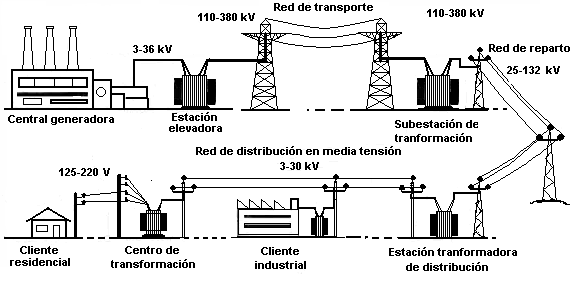
\includegraphics[width=0.9\textwidth]{figures/red_distribucion.png}
	\caption{Sistema de suministro eléctrico tradicional. Fuente: \cite{red-distribucion}}
\end{figure}

\section{Técnicas de Aprendizaje Automático}

El aprendizaje automático es una rama de la inteligencia artificial cuyo objetivo es el estudio y desarrollo de sistemas capaces de adaptar su comportamiento a partir de la experiencia. Para construir dicha experiencia, el sistema aplica un algoritmo de aprendizaje sobre un conjunto de ejemplos de entrenamiento, dotando al sistema de la capacidad de aprender y predecir resultados sin necesidad de una programación explícita. 

Existen diversos tipos de algoritmos de aprendizaje automático, que pueden clasificarse en general en cuatro categorías principales:
\begin{itemize}
	\item \textbf{Aprendizaje supervisado:} El sistema se entrena con un conjunto de datos etiquetados. Cada ejemplo se describe mediante un conjunto de atributos de entrada o características y una salida objetivo conocida que define la salida pretendida por el sistema. El objetivo del modelo es aprender la relación entre las entradas y las salidas para predecir correctamente la salida de nuevos ejemplos.
	\item \textbf{Aprendizaje no supervisado:} El sistema se entrena con un conjunto de datos sin etiquetar. De cada ejemplo se desconoce la salida esperada, por lo tanto su objetivo es identificar patrones o estructuras en los datos que ayuden a organizarlos.
	\item \textbf{Aprendizaje semisupervisado:} El sistema se entrena con un conjunto de datos en el que solo una parte está etiquetada, lo que permite aprovechar tanto la información supervisada como la no supervisada para mejorar el rendimiento del modelo.
	\item \textbf{Aprendizaje por refuerzo:} El sistema aprende mediante la interacción con el entorno, tomando decisiones en una secuencia de estados y recibiendo recompensas o castigos según el resultado de sus acciones. El objetivo es elegir la mejor secuencia de acciones (política óptima) que maximiza la recompensa acumulada.
\end{itemize}

Este proyecto se centra en el uso de algoritmos de \textbf{aprendizaje supervisado}. Esta elección resulta la más adecuada dado que se dispone de un conjunto de datos etiquetados, que contiene tanto el estado de la red en cada instante (variables de entrada) como la salida objetivo correspondiente. Estos algoritmos se pueden subdividir en \textbf{clasificación}, cuando la variable objetivo referencia a un tipo discreto y en \textbf{regresión} cuando la variable objetivo referencia a un valor continuo. Considerando que los datos con los que se trabaja corresponden con valores de magnitudes físicas, típicamente voltaje e intensidad de corriente, los modelos desarrollados se centran en resolver un problema de regresión.

\subsection{Ciclo de Vida del Aprendizaje Automático}
Existen múltiples algoritmos y modelos de aprendizaje automático supervisado y aunque difieren en su arquitectura interna, comparten el objetivo común de ajustar una serie de \textbf{parámetros} a partir de los ejemplos de entrenamiento. En consecuencia, entrenar un modelo consiste en hallar la combinación óptima de los parámetros del algoritmo que minimice la diferencia entre las predicciones realizadas y los valores reales. Este proceso de ajuste consiste fundamentalmente en minimizar una \textbf{función de pérdida} que mide la distancia entre las predicciones realizadas por el modelo y los datos de entrenamiento. La elección de una función de pérdida adecuada es crítica y depende de la naturaleza de la tarea a resolver.

\begin{figure}[htp]
	\centering
	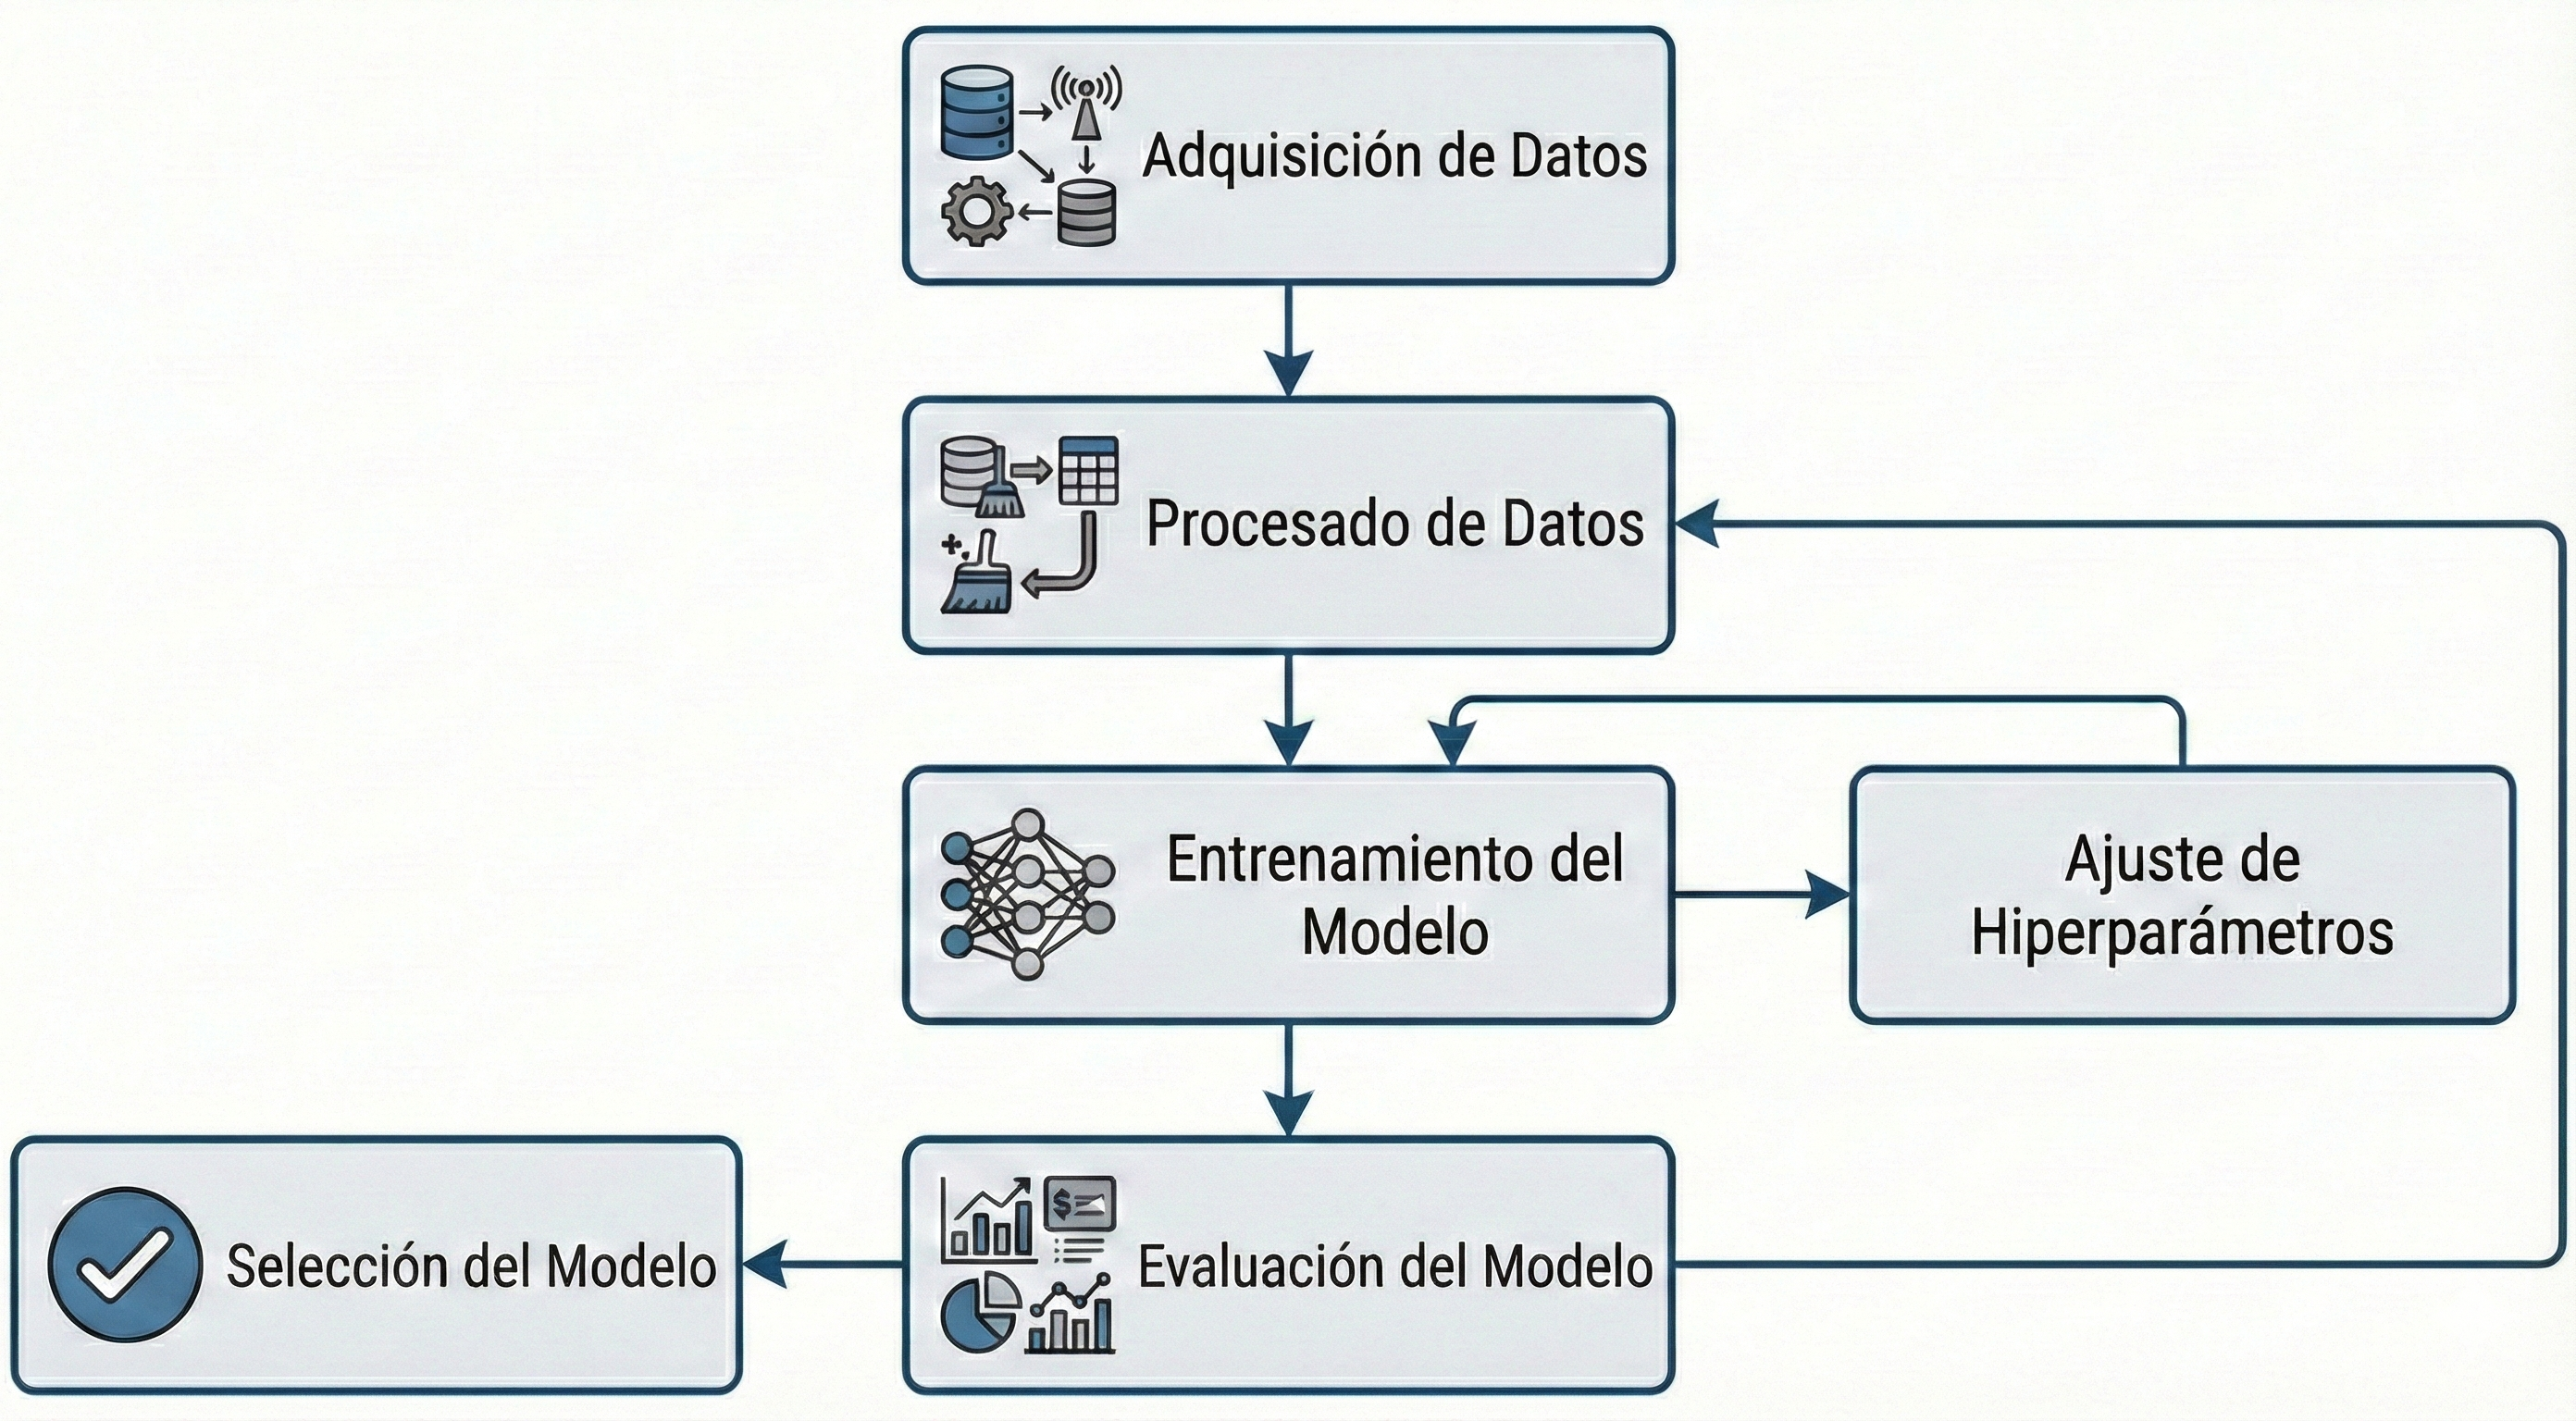
\includegraphics[width=0.9\textwidth]{figures/ciclo_vida_machine_learning.png}
	\caption{Principales procesos del aprendizaje automático. Fuente: Elaboración propia}
\end{figure}

Para que el entrenamiento sea efectivo y el modelo alcance una capacidad de generalización satisfactoria, es necesario disponer de una gran cantidad de datos. La cantidad necesaria de datos varía en función de la complejidad del modelo y principalmente de la naturaleza del problema (no es lo mismo tratar de aprender un comportamiento no lineal que uno lineal). Otro aspecto relevante es la calidad de los datos. Si el \textit{dataset} de entrenamiento contiene errores o ruido, será más complicado para el modelo detectar patrones subyacentes. Además, los datos deberán ser representativos del dominio del problema que se pretende modelar, teniendo gran importancia la manera en que se trabajan estos datos para no incurrir en sesgos de muestreo.

Unos de los mayores desafíos en el entrenamiento es evitar el \textbf{\textit{overfitting} (sobreajuste)} y el \textbf{\textit{underfitting} (subajuste)}. El sobreajuste se produce cuando el modelo se ajusta excesivamente a los datos de entrenamiento, llegando a memorizar el ruido aleatorio en lugar de aprender la tendencia subyacente. Esto resulta en una capacidad de generalización deficiente ante nuevos datos. Por el contrario, el subajuste ocurre cuando el modelo es demasiado simple o rígido para capturar la estructura y complejidad de los datos, generando predicciones imprecisas. Por tanto, el objetivo final es encontrar un punto óptimo de complejidad que permita al modelo aprender los patrones relevantes sin asimilar el ruido, garantizando así predicciones robustas y fiables ante nuevos datos.

\begin{figure}[htp]
	\centering
	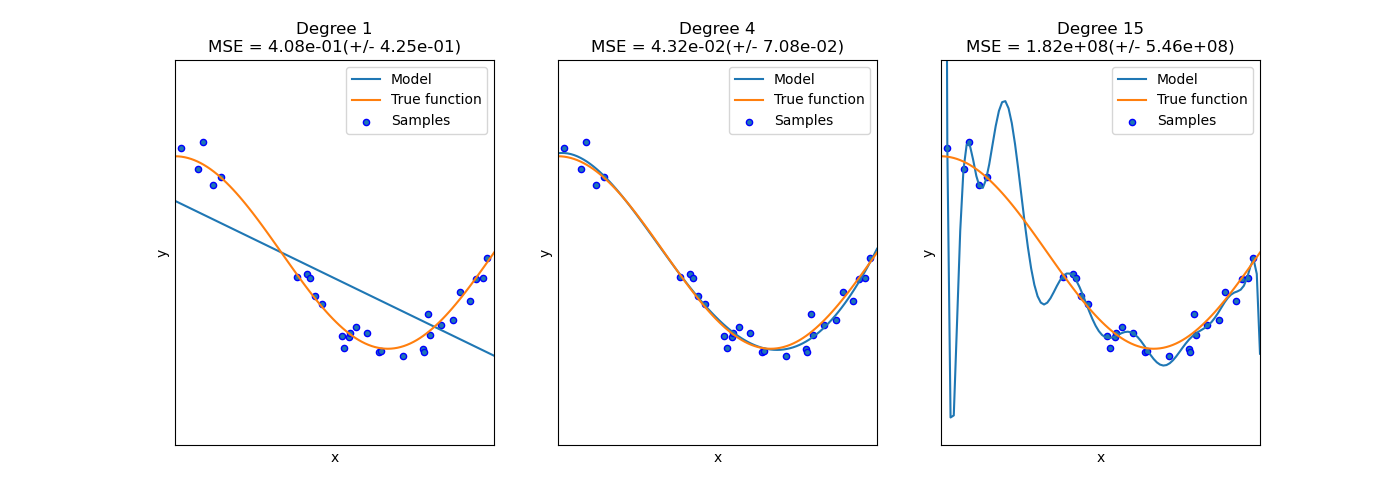
\includegraphics[width=0.9\textwidth]{figures/sobreajuste_subajuste.png}
	\caption{Ejemplos de subajuste, buen ajuste y sobreajuste. Fuente: \cite{scikit-learn-over-under}}
\end{figure}

Otro punto crítico en el entrenamiento de modelos es la \textbf{optimización de hiperparámetros}. Los hiperparámetros son variables de configuración externa que son prefijados de antemano y a diferencia de los parámetros, estos no se ajustan de manera automática durante el proceso de aprendizaje. Es fundamental en toda actividad del aprendizaje automático la selección de un buen conjunto de hiperparámetros, ya que estos controlan de forma directa la estructura, funciones y rendimiento de los modelos. No hay reglas establecidas en cuanto a qué hiperparámetros funcionan mejor ni sobre sus valores óptimos. Es necesario experimentar para encontrar la configuración óptima. Esta actividad se conoce como ajuste de hiperparámetros u optimización de hiperparámetros \cite{aws-hiperparam}. Este ajuste resulta relevante para evitar el sobreajuste y subajuste, ya que establecen restricciones para los modelos, permitiendo un mayor o menor ajuste a los datos de entrenamiento.

El propósito fundamental de todo modelo de aprendizaje automático reside en la resolución eficaz de un problema específico. En consecuencia, la \textbf{validación del modelo} constituye una fase crítica para garantizar su aptitud. Este proceso requiere la definición de \textbf{métricas de evaluación} cuantitativas que midan ese rendimiento. La selección de las métricas dependerá de las dimensiones del rendimiento que se deseen priorizar.

Para un cálculo riguroso de métricas de evaluación, es indispensable realizar una partición del conjunto de datos original en dos subconjuntos independientes: uno destinado al entrenamiento y otro a dicho cálculo. Esta metodología proporciona una evaluación objetiva con datos no vistos previamente por el modelo, simulando el comportamiento que tendrá el sistema en un entorno real. Dicha separación resulta esencial para detectar el sobreajuste, asegurando así que los resultados reflejen una verdadera capacidad de generalización del modelo y no la mera memorización de los patrones procesados. En siguientes secciones se exploran las metodologías utilizadas para la selección de ese conjunto de prueba.

\subsection{Modelos de Aprendizaje Automático}
Atendiendo a la naturaleza de regresión del problema, en esta sección se presentan los algoritmos que componen este estudio.

\subsubsection{Random Forest}
El modelo \textit{random forest} (bosque aleatorio) es un algoritmo de aprendizaje supervisado que se fundamenta en el paradigma de los \textbf{\textit{ensemble methods} (métodos por conjuntos)}. Puede ser utilizado tanto en tareas de clasificación como de regresión. A diferencia de los modelos tradicionales que buscan construir un único predictor robusto, las técnicas de ensamblaje combinan las predicciones de múltiples modelos base, denominados \textit{weak learners} (estimadores débiles), para obtener un resultado final más preciso y estable. Esta técnica de ensamble de modelos será muy relevante para el desarrollo del proyecto.

\begin{figure}[htp]
	\centering
	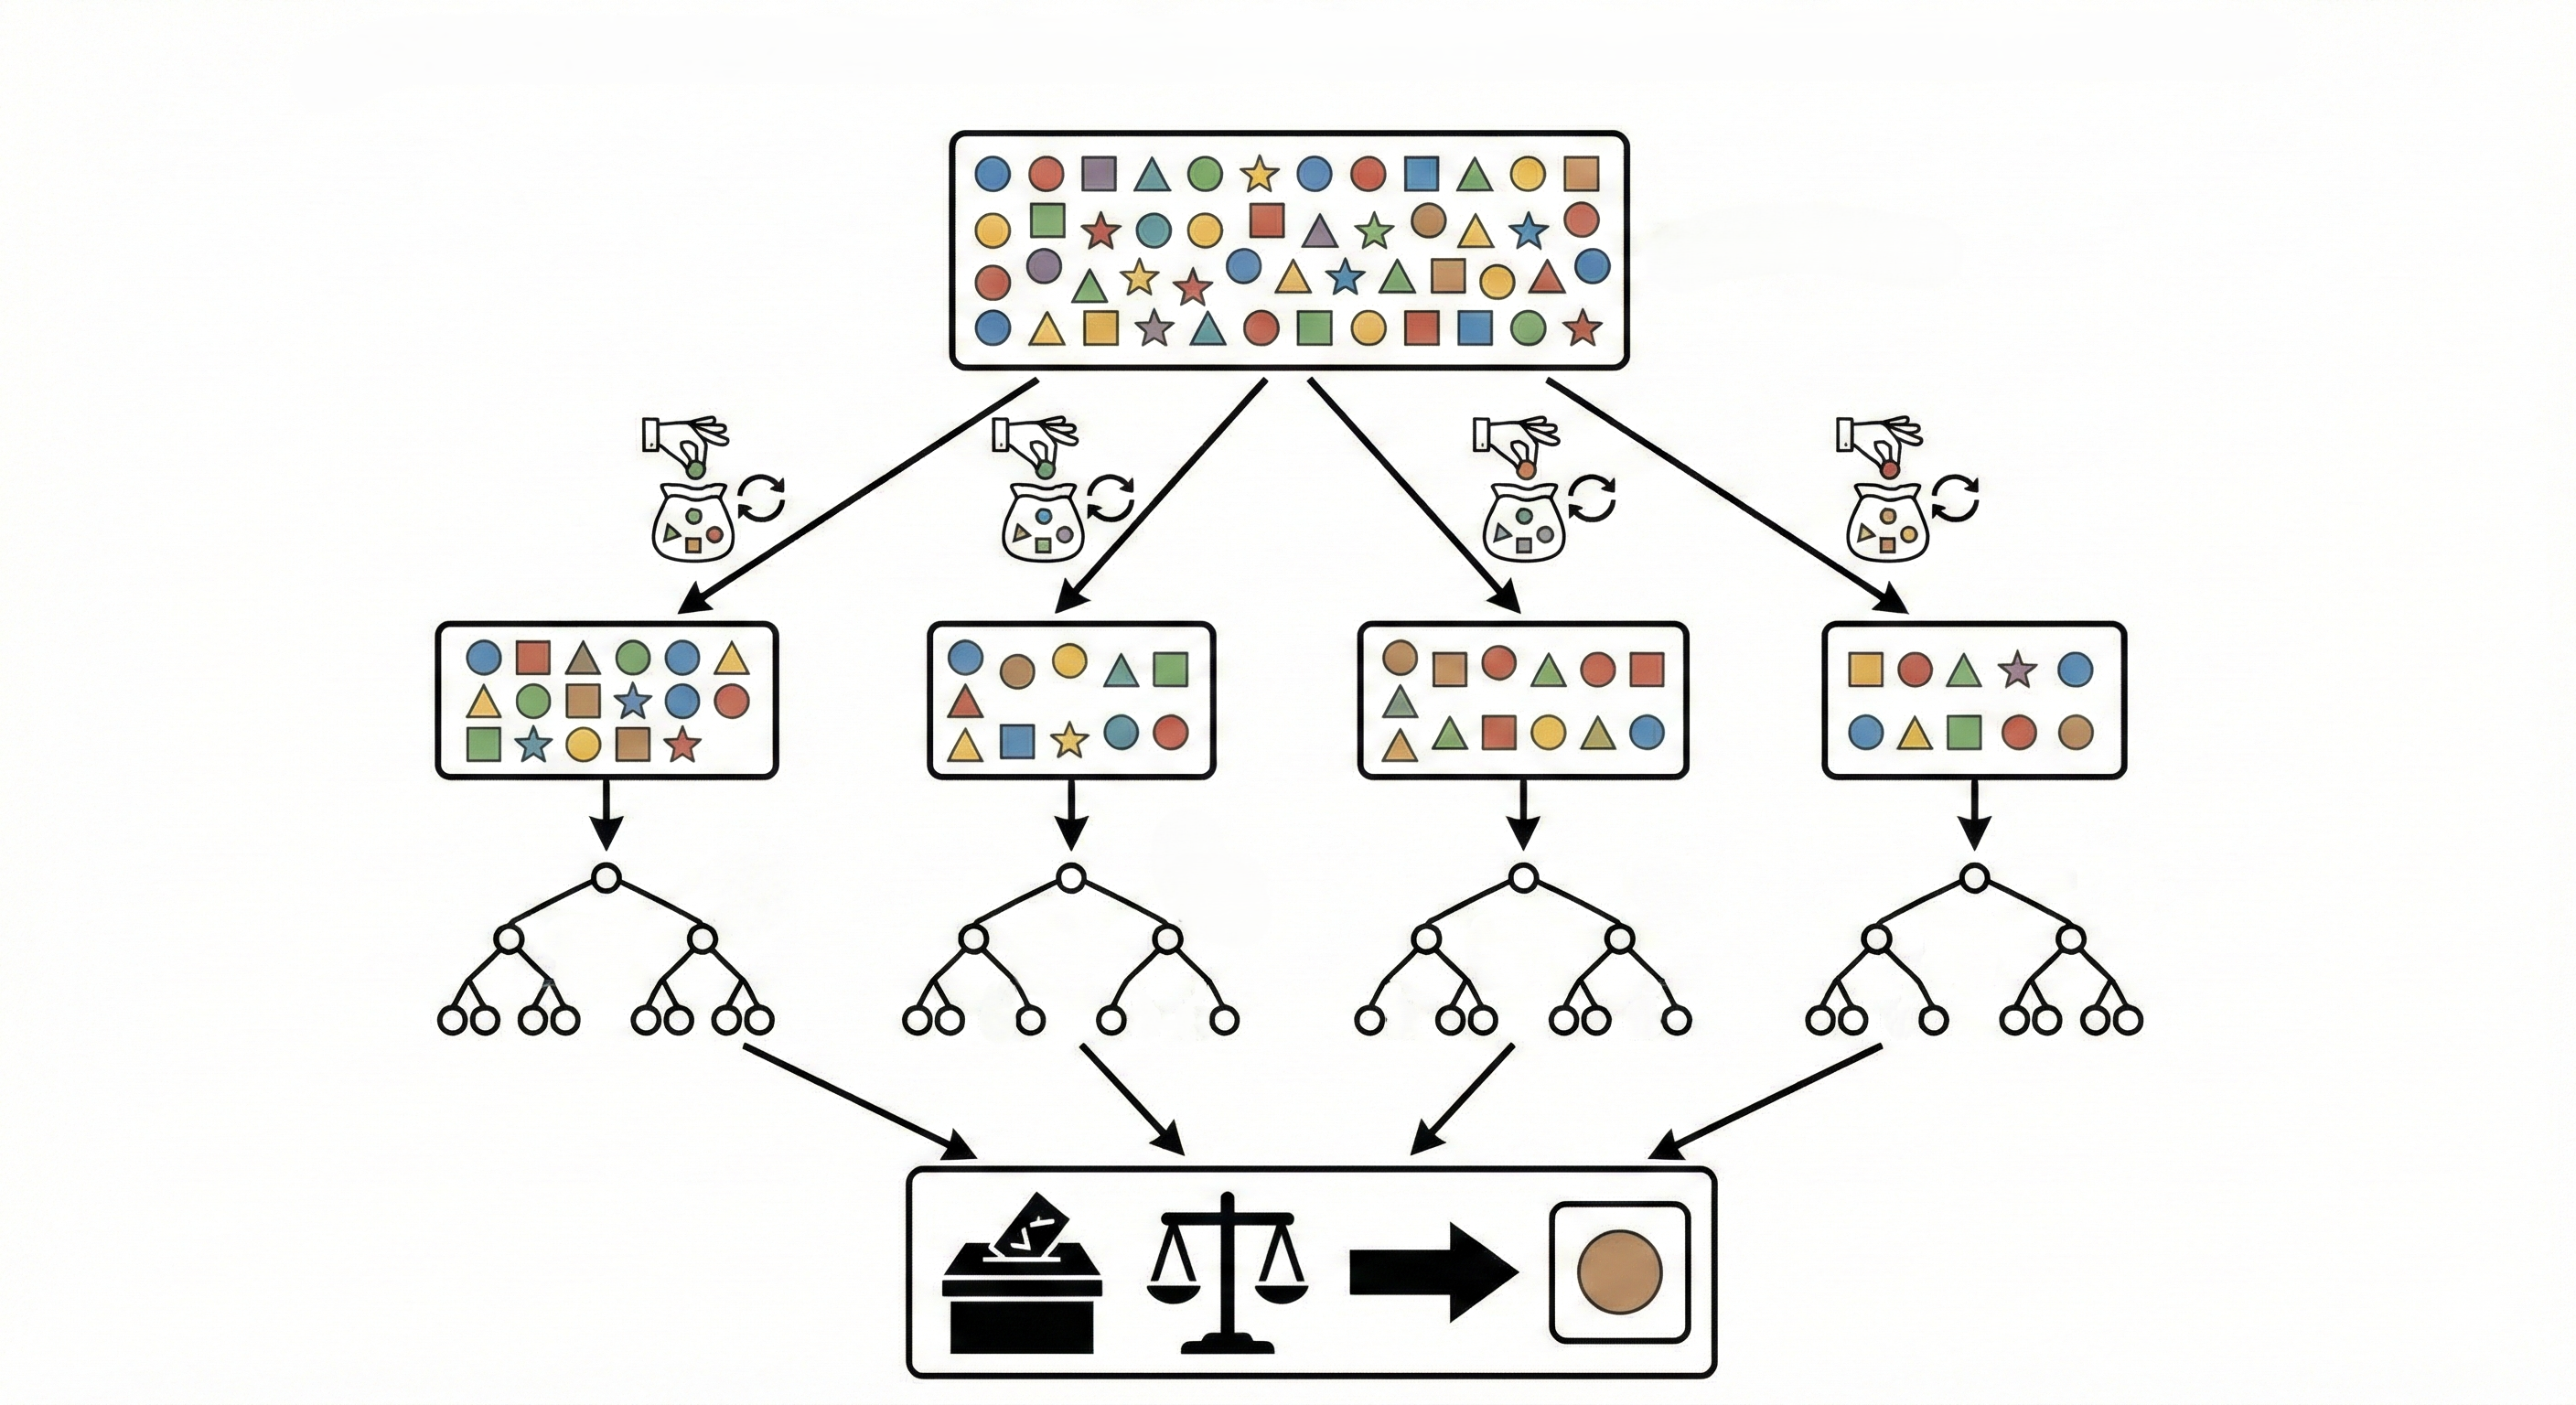
\includegraphics[width=0.9\textwidth]{figures/random_forest.png}
	\caption{Esquema de Random Forest y técnica de Bagging. Fuente: Elaboración propia}
\end{figure}

El enfoque de la técnica de ensamblaje se basa en la inteligencia colectiva. La agregación de múltiples modelos, que individualmente pueden tener un alto sesgo, tiende a compensar los errores individuales. En el caso del \textit{Random Forest}, este ensamble se construye utilizando \textbf{\textit{decision trees} (árboles de decisión)} como estimadores débiles, aplicando una técnica conocida como \textit{bagging (ensamblado mediante remuestreo)} \cite{ibm-bagging}. Esta técnica aplicada al \textit{Random Forest}, consiste en generar múltiples subconjuntos de entrenamiento del mismo tamaño que el conjunto de datos original. Este proceso se realiza mediante un muestreo aleatorio, en el que una misma instancia puede estar presente varias veces en un subconjunto y quedar excluida en otro. Posteriormente se entrena un \textit{Decision Tree} para cada una de estas muestras con los mismos hiperparámetros establecidos. Los modelos resultantes, por tanto, diferirán en sus parámetros, en este caso, su estructura interna. Finalmente, en problemas de regresión, la predicción del modelo global se obtiene promediando las salidas de los modelos débiles. Esta estrategia mitiga significativamente el sobreajuste y reduce la varianza, asumiendo a cambio un mayor coste computacional proporcional al número de estimadores utilizados.

El \textit{Decision Tree}, algoritmo base sobre el que se fundamenta \textit{Random Forest}, es un modelo ampliamente adoptado en el aprendizaje automático debido principalmente a su interpretabilidad y versatilidad. Es un algoritmo no paramétrico cuyo fundamento teórico responde a la estrategia "divide y vencerás". El modelo estructura la toma de decisiones mediante un grafo acíclico dirigido (árbol dirigido), organizando reglas lógicas secuenciales que divide el espacio de datos en regiones disjuntas. El proceso de construcción del árbol (entrenamiento) se realiza mediante un enfoque voraz y recursivo: en cada iteración, el algoritmo selecciona la partición óptima que mejor discrimina la variable objetivo. Este proceso continúa hasta satisfacer un criterio de parada predefinido, tal como alcanzar una profundidad máxima, un número mínimo de muestras por nodo o un umbral de varianza (impureza) específico.

\begin{figure}[htp]
	\centering
	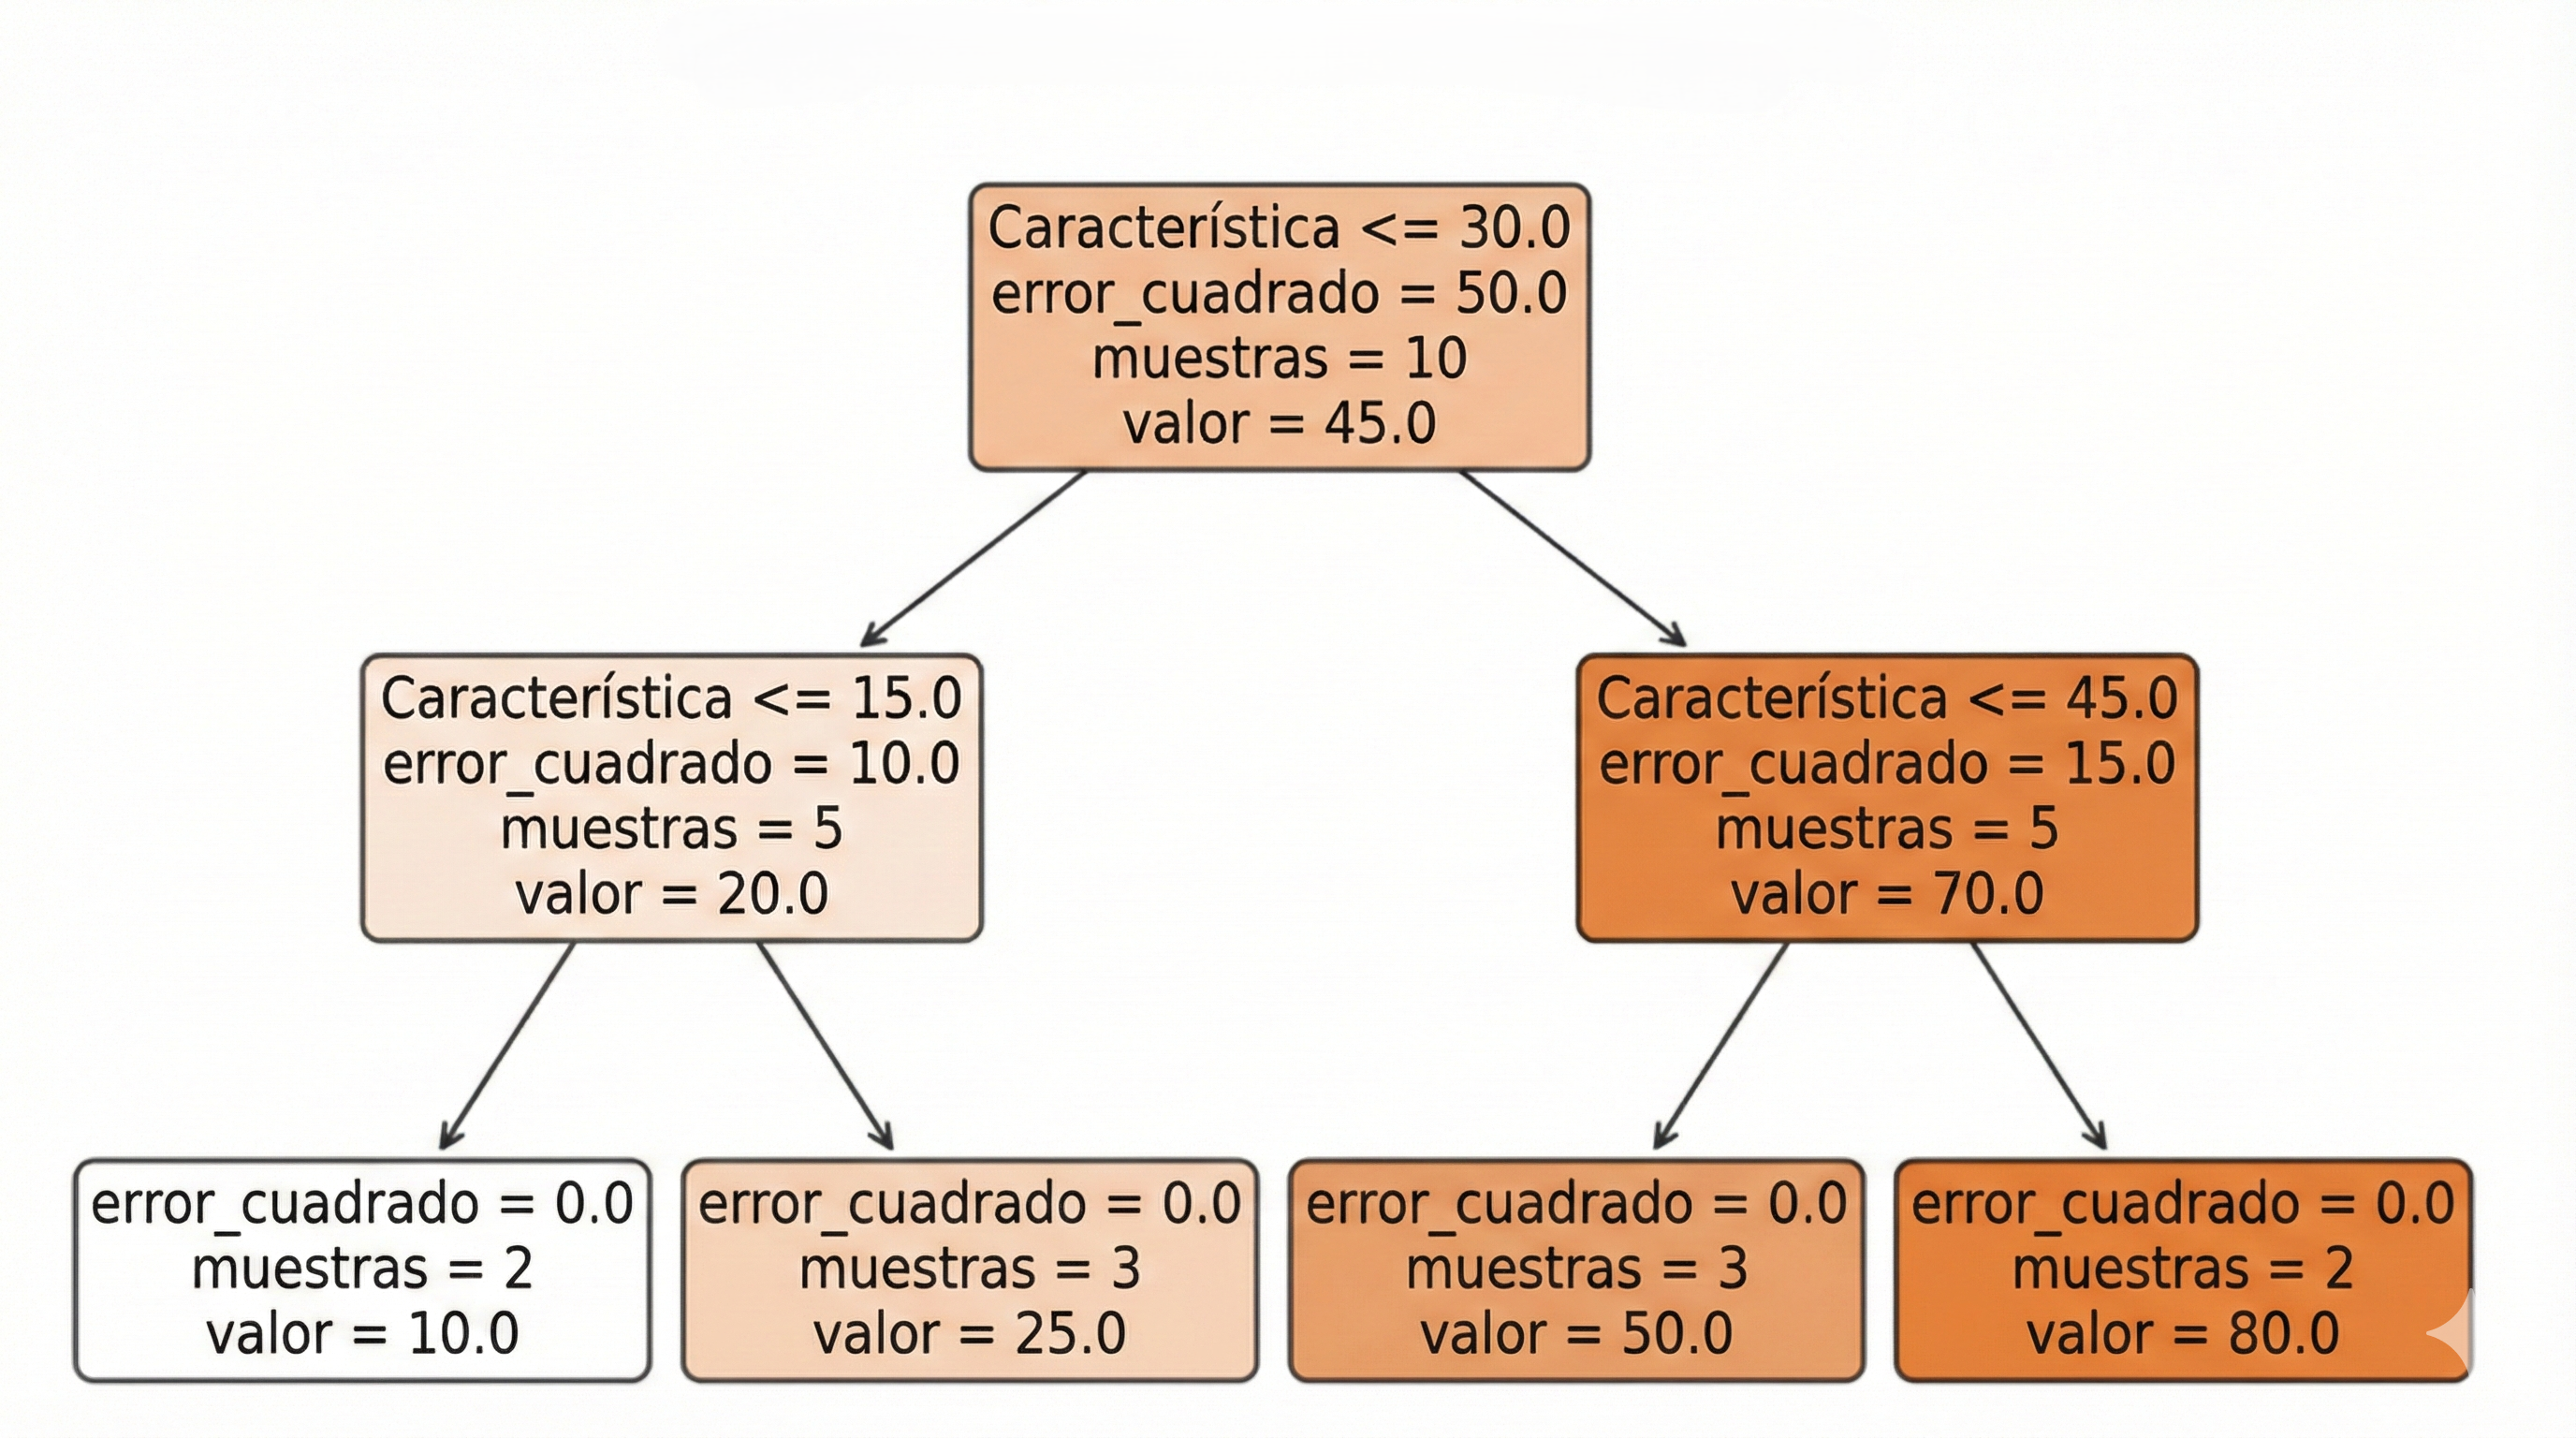
\includegraphics[width=0.6\textwidth]{figures/decision_tree.png}
	\caption{Esquema de Decision Tree. Fuente: Elaboración propia}
\end{figure}

\subsubsection{XGBoost}
\textit{eXtreme Gradient Boosting} (XGBoost) es una librería de aprendizaje automático open source (código abierto) basada en la técnica \textbf{\textit{gradient boosting} (potenciación por el gradiente)} \cite{xgboost}. Esta metodología se basa de nuevo en los métodos por conjuntos, pero a diferencia del \textit{Random Forest} con un enfoque de ensamblaje paralelo, adopta una estrategia secuencial y aditiva. 

En lugar de entrenar modelos independientes, la potenciación por el gradiente construye una cadena de estimadores débiles, típicamente \textit{Decision Trees}, donde cada nuevo modelo se diseña específicamente para corregir los \textbf{errores residuales} cometidos por la suma de los modelos anteriores. El término ``gradiente'' alude al mecanismo matemático de optimización subyacente: el algoritmo minimiza una \textbf{\textit{loss function} (función de pérdida)} diferenciable. En cada iteración, el nuevo árbol se ajusta en la dirección del gradiente negativo de la función de pérdida respecto a la predicción actual, lo que permite refinar progresivamente la precisión del modelo global.

\begin{figure}[htp]
	\centering
	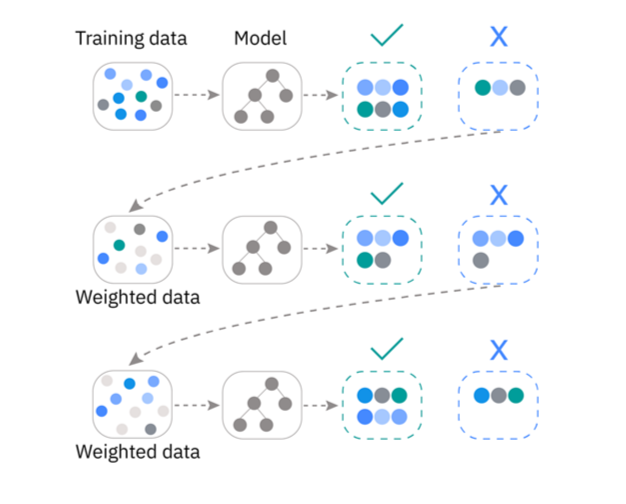
\includegraphics[width=0.4\textwidth]{figures/xgboost.png}
	\caption{Esquema de XGBoost. Fuente: \cite{xgboost_ibm}}
\end{figure}

\subsubsection{Redes Neuronales}
Una red neuronal es un algoritmo basado en un proceso denominado \textbf{\textit{deep learning} (aprendizaje profundo)}, que utiliza nodos o neuronas artificiales interconectados en una estructura de capas que simula el comportamiento del cerebro humano. Las redes neuronales gozan de una amplia popularidad, ya que son capaces de aprender estructuras y comportamientos complejos. Son algoritmos muy usados en reconocimiento de imágenes, procesamiento del lenguaje natural o previsión de la carga eléctrica y demanda de energía entre otros \cite{aws-red-neuro}.

La unidad mínima de procesamiento son neuronas o nodos, que están estructuradas en capas. Cada nodo recibe una entrada, la procesa y manda el resultado a nodos de la siguiente capa. Cada transferencia de una neurona previa a una posterior es modulada por un peso, que son los parámetros que el algoritmo debe aprender.

Una red neuronal básica consta de tres capas:
\begin{itemize}
	\item \textbf{Capa de entrada:} La información exterior entra en la red neuronal artificial por esta capa, donde se procesan los datos y se pasan a la siguiente capa.
	\item \textbf{Capa oculta:} Toman su entrada de la capa de entrada o de otras capas ocultas. Esta capa es la que realiza la tarea de aprendizaje.
	\item \textbf{Capa de salida:} Proporciona el resultado final de todo el procesamiento de datos que realiza la red neuronal. Puede tener uno o varios nodos de salida.
\end{itemize}

\begin{figure}[htp]
	\centering
	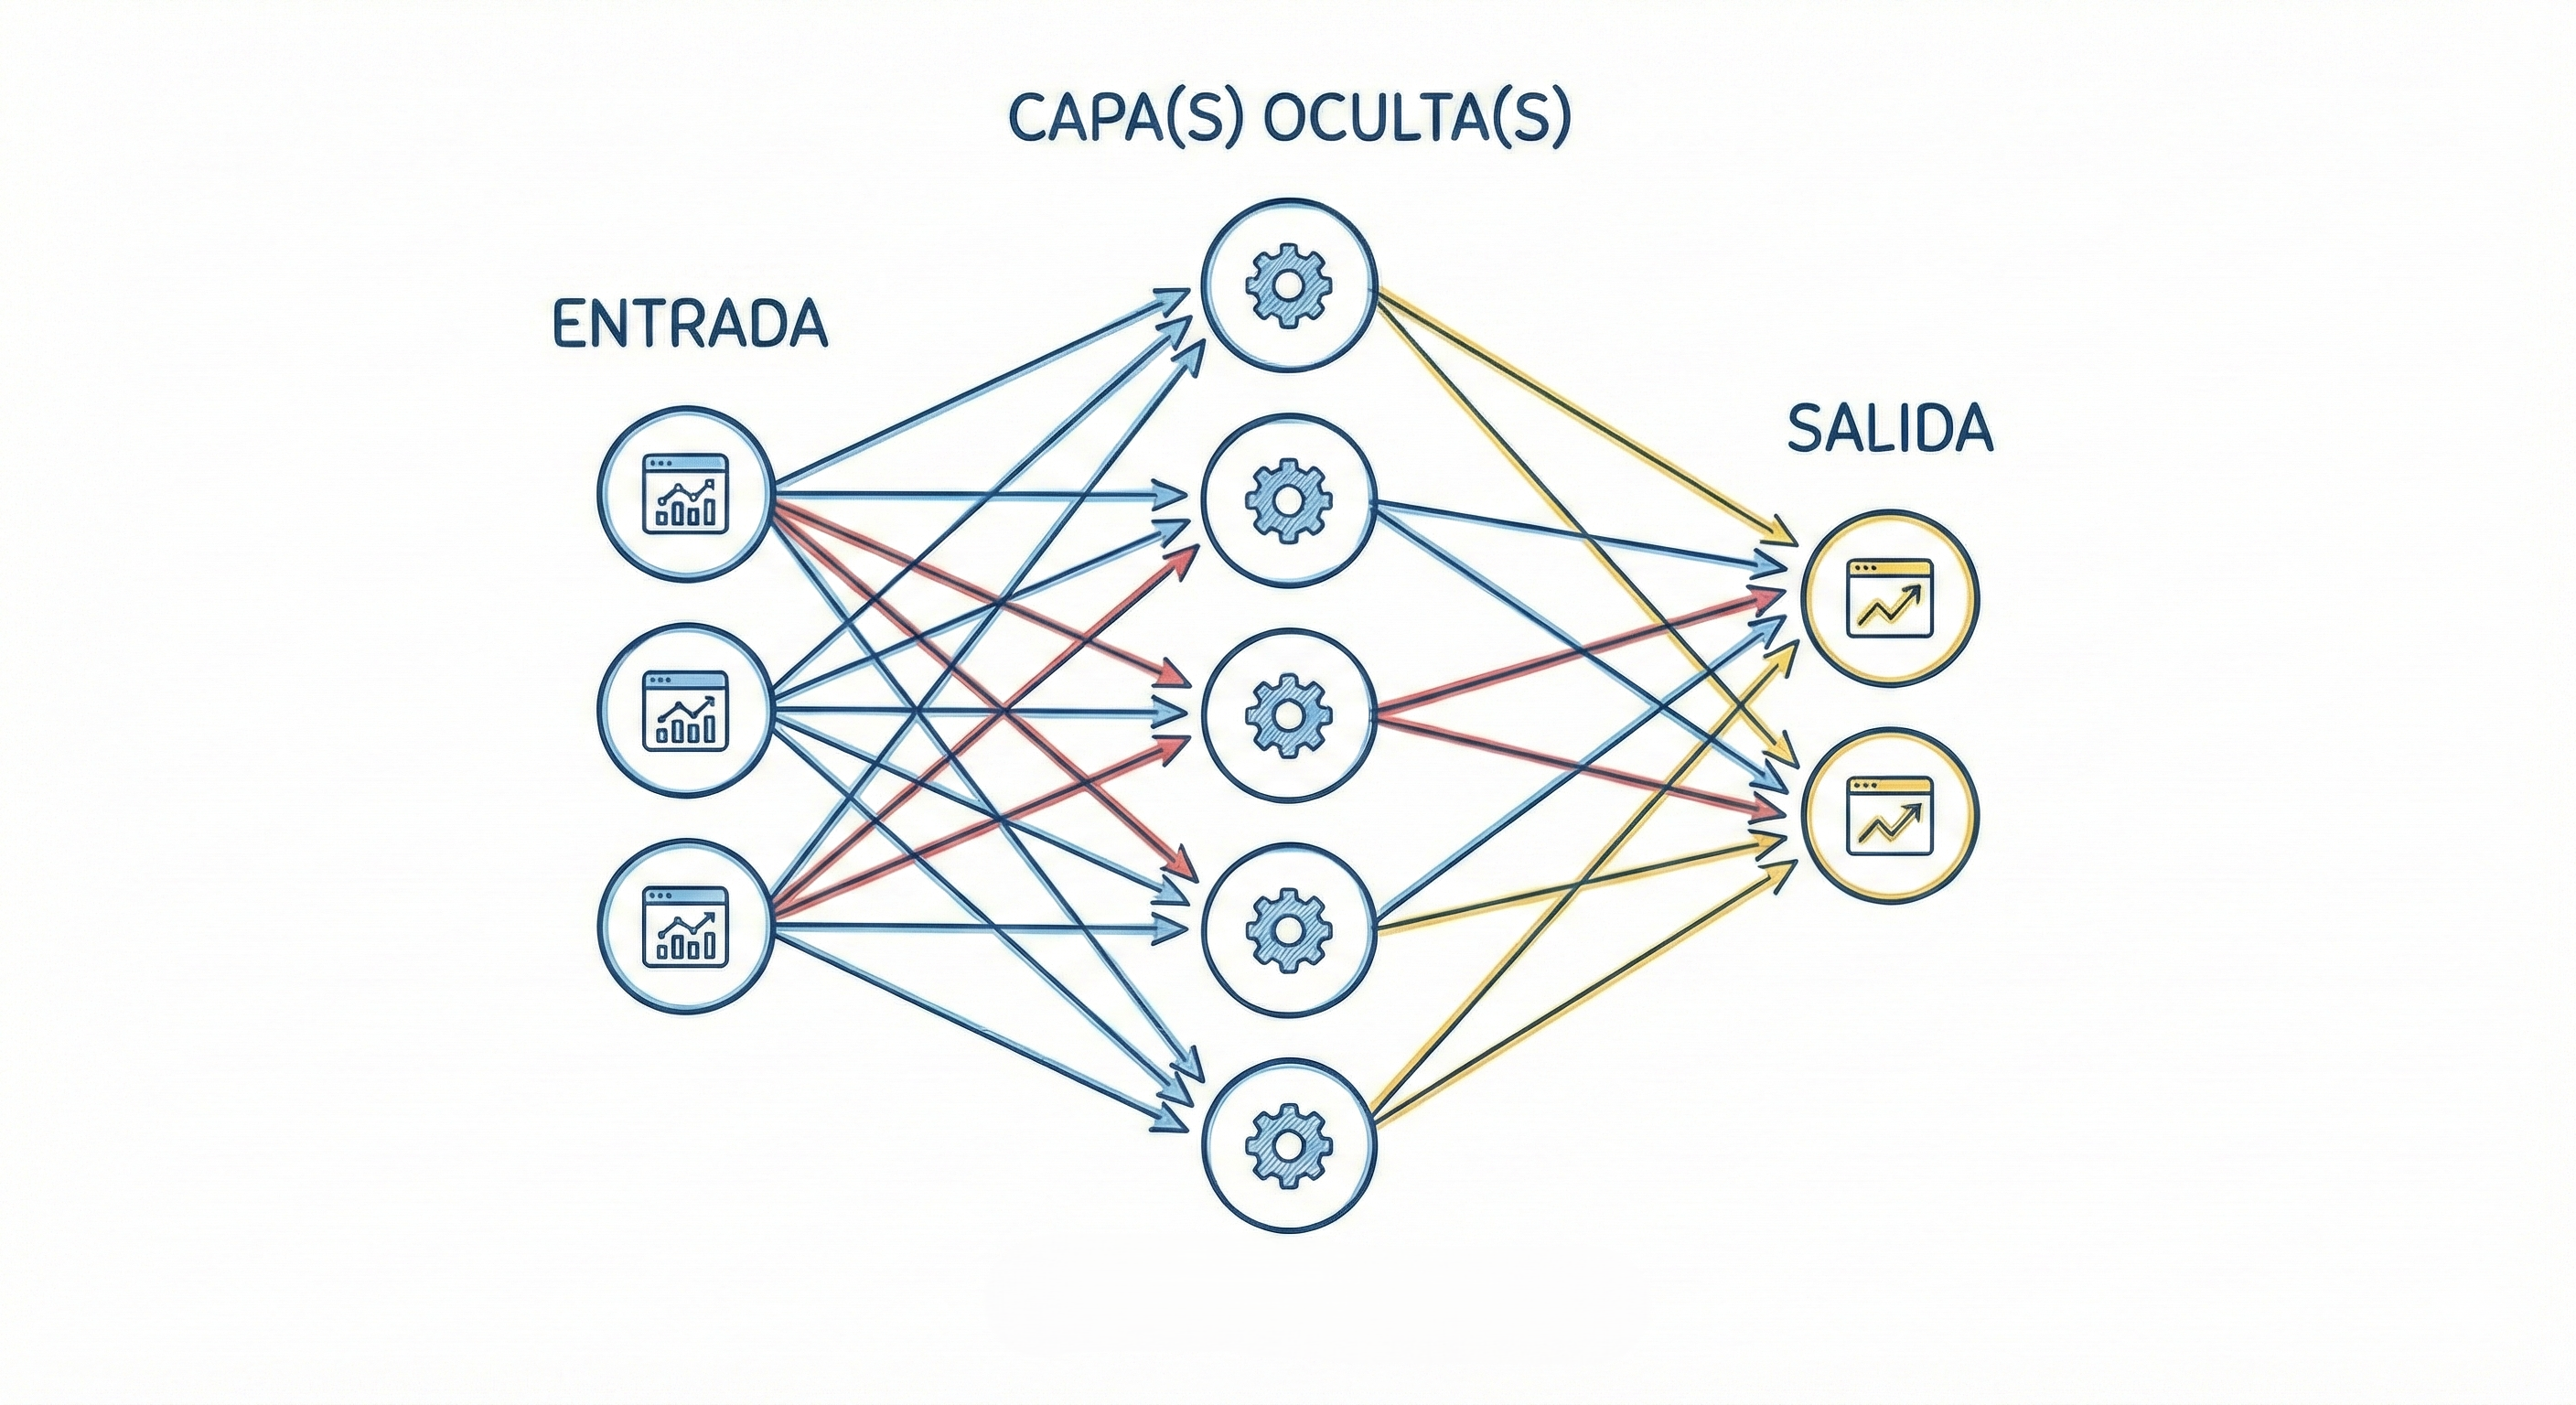
\includegraphics[width=0.9\textwidth]{figures/redes_neuronales.png}
	\caption{Estructura de una Red Neuronal. Fuente: Elaboración propia}
\end{figure}

Para entrenar una red neuronal, cada neurona calcula:
\begin{equation}
	a = \sigma(W^TX + b)
\end{equation}
Donde \textit{\textbf{X}} es el vector de los argumentos, \textit{\textbf{W}} es el vector de pesos asociados a los argumentos, \textit{\textbf{b}} es el sesgo de activación, $\boldsymbol{\sigma}$ es la función de activación y \textit{\textbf{a}} es la salida \cite{o-reilly-machine-learning}. La función de activación y el sesgo tienen como objetivo determinar si la neurona debe o no activarse. Esta característica es la que permite a las redes neuronales aprender patrones complejos. Las redes neuronales profundas, tienen varias capas ocultas con millones de neuronas artificiales conectadas entre sí. En teoría, estas redes pueden asignar cualquier tipo de entrada a cualquier tipo de salida. Sin embargo, también necesitan mucho más entrenamiento en comparación a otros modelos y millones de ejemplos de datos de entrenamiento.

El entrenamiento de una neurona artificial, como modelo de regresión, se realiza minimizando una función de pérdida o coste utilizando un método de optimización como el descenso por el gradiente. Para minimizar esta pérdida, el método estándar es el algoritmo de \textbf{\textit{backpropagation} (retropropagación)}. Este algoritmo aplica recursivamente la regla de la cadena para calcular las derivadas parciales de manera eficiente de la función de coste respecto a los pesos. 

Las redes neuronales han evolucionado hacia arquitecturas especializadas adecuadas para diferentes dominios. Entre los diferentes tipos de arquitecturas se pueden destacar:
\begin{itemize}
	\item \textbf{Redes neuronales convolucionales:} Están diseñadas principalmente para el procesamiento de imágenes. Destacan en el reconocimiento de imágenes, la visión artificial y el reconocimiento facial gracias a filtros convolucionales.
	\item \textbf{Redes neuronales recurrentes:} Incorporan bucles de \textit{feedback} que permiten que la información persista a lo largo de los pasos temporales. Son adecuados para el reconocimiento de voz, la previsión de series temporales y los datos secuenciales.
	\item \textbf{Transformadores:} Una arquitectura moderna, que aprovecha mecanismos de atención para capturar dependencias en el procesamiento del lenguaje natural y potencian modelos de última generación como GPT.
\end{itemize}

\subsubsection{Otras Opciones}
En este trabajo se ha profundizado en los modelos secuenciales y redes neuronales, debido a su robustez y su consolidación como el estándar en la industria. Sin embargo, cabe destacar la existencia de otros algoritmos. 

Las \textbf{Máquinas de Vectores de Soporte (SVM)} son eficaces en espacios de alta dimensionalidad, mientras que implementaciones modernas de \textit{boosting} como \textit{\textbf{LightGBM}} o \textit{\textbf{CatBoost}} ofrecen mejoras en eficiencia computacional y manejo de variables categóricas.

Las SVM presentan limitaciones importantes de escalabilidad, ya que su coste computacional y de memoria crece de forma cuadrática con el volumen de datos. Esto las hace poco viables para grandes conjuntos de datos. Además, no capturan de forma natural la secuencialidad de los datos sin un preprocesamiento exhaustivo. 

De igual forma, las implementaciones de LightGBM y CatBoost asumen que las observaciones son independientes entre sí. Para aplicarlos a problemas temporales, estos modelos requieren un diseño manual de características muy laborioso.

La elección final del modelo no debe basarse únicamente en la potencia bruta. No existe un algoritmo universal superior para todos los problemas. La selección depende del compromiso entre precisión, interpretabilidad, volumen de datos y recursos computacionales disponibles.

\subsection{Aplicación del Aprendizaje Automático en Redes Eléctricas}
En los últimos años, la aplicación de técnicas de aprendizaje automático ha cobrado un gran protagonismo en la operación de las redes eléctricas inteligentes para abordar desafíos exigentes. En muchos casos, estas aplicaciones superan con creces las capacidades de los sistemas de gestión convencionales \cite{useful-application-smart-grids-ieee}. Al dotar a la infraestructura de inteligencia, se facilita la transición de un modelo eléctrico pasivo a uno dinámico y bidireccional.

Entre las áreas de aplicación más maduras destaca la predicción de demanda y generación energética. El uso de modelos basados en algoritmos predictivos y aprendizaje profundo permite analizar grandes conjuntos de datos históricos, patrones de consumo y variables meteorológicas para predecir fluctuaciones a corto y medio plazo. Esto resulta fundamental para equilibrar con gran precisión la inyección de fuentes de energía renovables, cuya naturaleza es inherentemente intermitente \cite{load-forecasting-2024}.

Del mismo modo, estas técnicas están revolucionando la adaptabilidad y la seguridad de la infraestructura mediante la detección y el diagnóstico de fallos en la red. Algoritmos de clasificación basados en \textit{Random Forest} o la potenciación por gradiente se emplean actualmente para monitorizar el estado de los componentes en tiempo real. Esta monitorización posibilita el mantenimiento predictivo y facilita el aislamiento automático de averías. Esta característica conocida como \textit{self-healing} (autorrecuperación) logra un tiempo de respuesta y una precisión muy superiores a las inspecciones tradicionales \cite{fault-detection-2024}.

Más allá de la predicción pasiva y la monitorización de anomalías, el verdadero reto actual reside en el control activo de la red, el cual requiere optimizar parámetros físicos complejos en tiempos computacionales muy reducidos. Tradicionalmente, problemas determinantes como el flujo de cargas óptimo o la regulación de tensiones nodales se han abordado mediante modelos matemáticos deterministas, estáticos y altamente no lineales. Sin embargo, revisiones recientes en la literatura destacan cómo los enfoques basados en datos logran aproximar estas soluciones matemáticas de forma casi instantánea una vez que los modelos están entrenados. De esta forma, se adaptan mucho mejor a la alta variabilidad que introducen los recursos energéticos distribuidos \cite{review-machine-learning}.

Asimismo, los métodos tradicionales de OPF centralizados presentan graves cuellos de botella en términos de escalabilidad y comunicaciones al aplicarse a redes inteligentes de gran tamaño. Como respuesta, la comunidad investigadora está explorando activamente arquitecturas algorítmicas distribuidas que aligeran la carga de procesamiento y protegen la privacidad de los datos locales de los nodos \cite{distributed-opf-ieee}.

Es exactamente en este contexto donde se enmarca el presente proyecto, apoyándose en la capacidad de los modelos de aprendizaje automático para resolver problemas no lineales complejos. Este trabajo propone una arquitectura capaz de fusionar dos necesidades críticas de las redes modernas: la estimación rápida y precisa del estado de la red, y el control activo de sus variables físicas mediante la inyección óptima de potencia reactiva.
    \chapter{Objetivos}\label{cap:objetivos}

El objetivo del presente Trabajo Fin de Grado consiste en desarrollar y evaluar diferentes modelos de Inteligenia Artificial mediante aprendizaje supervisado, capaces de predecir valores de referencia (set points) que optimicen el funcionamiento de redes eléctricas de distribución. El propósito de estos modelos será predecir de manera efectiva y precisa estos valores de referencia, reduciendo la necesidad de disponer de información detallada sobre la topología y parámetros eléctricos de la red, requeridos por métodos tradicionales de optimización como el algoritmo Optimal Power Flow. Con este fin, el entrenamiento de estos modelos se realizarán a partir de grandes volúmenes de datos medidos por sensores instalados en la red.

Para alcanzar este objetivo general, se plantean los siguientes objetivos específicos:
\begin{enumerate}
	\item \textbf{Análisis e Investigación de Tecnologías:} Seleccionar las librerías y frameworks de Inteligencia Artificial a utilizar y realizar un análisis e investigación exhaustiva de estas tecnologías, para una correcta implementación y optimización de los modelos predictivos en el contexto eléctrico.
	\item \textbf{Ingeniería de Datos y Preprocesamiento:} Tratar el dataset disponible mediante tareas de limpieza, normalización y transformación, aplicando técnicas de selección de características (Feature Selection), para reducir la dimensionalidad y garantizar la calidad de los datos de entrada de los modelos.
	\item \textbf{Construcción y Entrenamiento de Modelos Predictivos:} Desarrollar y entrenar arquitecturas de aprendizaje supervisado basadas en Random Forest, XGBoost y Redes Neuronales que se adapten a la problemática.
	\item \textbf{Optimización de Hiperparámetros:} Aplicar estrategias de optimización de hiperparámetros sobre los modelos implementados, para maximizar métricas de rendimiento y evitar el sobreajuste (overfitting).
	\item \textbf{Evaluación y Análisis Comparativo:} Evaluar el desempeño de los modelos utilizando métricas estadísticas rigurosas sobre conjuntos de datos de prueba no vistos anteriormente por los modelos, para realizar una comparación técnica entre estos y permitir una reflexión sobre su aplicabilidad real en contextos eléctricos.
\end{enumerate}
    \chapter{Análisis}\label{cap:analisis}
Este capítulo tiene como propósito fundamental traducir los objetivos generales y técnicos del proyecto en especificaciones formales que guíen el diseño y la posterior implementación del sistema. A continuación, se detallan los requisitos del sistema clasificados en generales, de información, funcionales y no funcionales.

\section{Requisitos Generales}
\begin{table}[htp]
	\centering
		\begin{tabular}{ | m{7cm} | m{8cm} | }
			\hline
			\rowcolor[HTML]{5B9BD5} 
			\textbf{Requisito General} & \textbf{Descripción}\\
			\hline
			
			RG-01: Creación del \textit{Pipeline} de \textit{Machine Learning} & El sistema debe componer un flujo de trabajo analítico de extremo a extremo que abarque desde la ingesta de los datos eléctricos brutos hasta la extracción de métricas de rendimiento, permitiendo la predicción del estado de la red \\
			\hline
			RG-02: Comparativa Tecnológica & El sistema debe estar diseñado de forma modular para permitir la evaluación y comparación justa entre diferentes paradigmas de aprendizaje automático \\
			\hline
			
		\end{tabular} 
		
		\caption{Requisitos generales del sistema}
	\end{table}
\clearpage

\section{Requisitos de Información}
\begin{table}[htp]
	\centering
	\renewcommand{\arraystretch}{1.3}
		\begin{tabular}{ | m{7cm} | m{8cm} | }
			\hline
			\rowcolor[HTML]{5B9BD5} 
			\textcolor{white}{\textbf{Requisito de Información}} & \textcolor{white}{\textbf{Descripción}}\\
			\hline
			
			RI-01: Datos de Entrada & El sistema debe ser capaz de procesar conjuntos de datos tabulares que representen el estado físico inicial de la red, concretamente las potencias activa y reactiva en los diferentes nudos eléctricos \\
			\hline
			RI-02: Datos de Salida & El sistema debe manejar y predecir de forma simultánea múltiples variables continuas correspondientes a la respuesta física de la red. Concretamente, las tensiones nodales, las pérdidas de potencia y la potencia reactiva inyectada por los generadores \\
			\hline
			RI-03: Modelos Predictivos & El sistema debe almacenar de forma automática los mejores modelos encontrados en las diferentes iteraciones para su posible uso en un entorno de producción \\
			\hline
			
		\end{tabular} 
		
		\caption{Requisitos de información del sistema}
	\end{table}

\section{Requisitos Funcionales}
\begin{table}[htp]
	\centering
		\begin{tabular}{ | m{7cm} | m{8cm} | }
			\hline
			\rowcolor[HTML]{5B9BD5} 
			\textbf{Requisito Funcional} & \textbf{Descripción}\\
			\hline
			
			RF-01: Procesado y Filtrado de Datos & El sistema debe cargar los datos provenientes del \textit{dataset} e identificar y descartar aquellos registros físicamente inconsistentes \\
			\hline
			RF-02: Transformación y Escalado & El sistema debe aplicar técnicas de normalización cuando sea necesario sobre las variables. Esta transformación debe ajustarse única y estrictamente sobre los conjuntos de datos de entrenamiento para prevenir el filtrado de información de los conjuntos de evaluación \\
			\hline
			RF-03: Entrenamiento de Algoritmos Estáticos & El sistema debe permitir instanciar, configurar y entrenar modelos basados en árboles de decisión, concretamente \textit{Random Forest} y \textit{XGBoost}, capaces de predecir simultáneamente variables con naturalezas distintas \\
			\hline 
			RF-04: Implementación de Redes Neuronales Multipropósito & El sistema debe ser capaz de construir arquitecturas de \textit{Deep Learning} con múltiples salidas independientes, permitiendo predecir simultáneamente variables con naturalezas distintas \\
			\hline
			RF-05: Arquitecturas Jerárquicas & El sistema debe soportar topologías de red secuenciales que respeten la causalidad física \\
			\hline
			RF-06: Búsqueda de Hiperparámetros & El sistema debe integrar módulos de optimización para explorar combinaciones de hiperparámetros que minimicen la función de pérdida seleccionada \\
			\hline
			RF-07: Validación Metodológica & El sistema debe dividir los datos empleando técnicas de retención para aislar un conjunto de validación final completamente ciego \\
			\hline
			RF-08: Cálculo de Métricas y Evaluación & El sistema debe calcular métricas de error absolutas y relativas directamente sobre las magnitudes reales para mostrar de forma objetiva y representativa la eficiencia de los modelos \\
			\hline
			RF-09: Visualización de Resultados & El sistema debe generar las gráficas pertinente para la contrastación de los resultados obtenidos por los modelos con el conjunto de validación final \\
			\hline
			
		\end{tabular} 
		
		\caption{Requisitos de información del sistema}
	\end{table}
\clearpage

\section{Requisitos No Funcionales}
\begin{table}[htp]
	\centering
		\begin{tabular}{ | p{7cm} | p{8cm} | }
			\hline
			\rowcolor[HTML]{90D5FF} 
			\textbf{Requisito de Información} & \textbf{Descripción}\\
			\hline
			
			RNF-01: Reproducibilidad Determinista & El sistema debe fijar semillas para garantizar que los experimentos sean completamente repetibles \\
			\hline
			RNF-02: Eficiencia computacional & La topología de los modelos y el tamaña de los lotes deben ser eficientes para que los tiempos de entrenamiento y optimización sean viables en un equipo informático con \textit{hardware} estándar, sin requerir equipo especializado de supercomputación \\
			\hline
			
		\end{tabular} 
		
		\caption{Requisitos de información del sistema}
	\end{table}

\section{Matriz de Trazabilidad}
%\begin{table}[htp]
	\centering
	\begin{tabular}{|m{5.5cm}|c|c|c|c|c|}
		\hline
		\rowcolor[HTML]{5B9BD5} 
		\textbf{Requisito \textbackslash\ Objetivo} & \textbf{OBJ-1} & \textbf{OBJ-2} & \textbf{OBJ-3} & \textbf{OBJ-4} & \textbf{OBJ-5} \\
		\hline
		\textbf{RG-01:} Creación del \textit{Pipeline} de \textit{Machine Learning} & & X & X & X & X \\
		\hline
		\textbf{RG-02:} Comparativa Tecnológica & X & & X & & X \\
		\hline
		\textbf{RI-01:} Datos de Entrada & & X & & & \\
		\hline
		\textbf{RI-02:} Datos de Salida & & X & & & \\
		\hline
		\textbf{RI-03:} Modelos Predictivos & & & X & & \\
		\hline
		\textbf{RF-01:} Procesado y Filtrado de Datos & & X & & & \\
		\hline
		\textbf{RF-02:} Transformación y Escalado & & X & & & \\
		\hline
		\textbf{RF-03:} Entrenamiento de Algoritmos Estáticos & & & X & & \\
		\hline
		\textbf{RF-04:} Implementación de Redes Neuronales Multipropósito & & & X & & \\
		\hline
		\textbf{RF-05:} Arquitecturas Jerárquicas & & & X & & \\
		\hline
		\textbf{RF-06:} Búsqueda de Hiperparámetros & & & & X & \\
		\hline
		\textbf{RF-07:} Validación Metodológica & & X & & & \\
		\hline
		\textbf{RF-08:} Cálculo de Métricas y Evaluación & & & & & X \\
		\hline
		\textbf{RF-07:} Visualización de Resultados & & & & & X \\
		\hline
		\textbf{RNF-01:} Reproducibilidad Determinista & & & X & X & X \\
		\hline
		\textbf{RNF-02:} Eficiencia Computacional & & & X & X & \\
		\hline
	\end{tabular}
	\caption{Matriz de trazabilidad de requisitos del sistema frente a los objetivos del proyecto}
\end{table}

\section{Planificación Temporal}
%TODO Planificación

\subsection{Tareas de Investigación}

\subsection{Tareas de Análisis}

\subsection{Tareas de Desarrollo}

\subsection{Tareas de Evaluación}

\subsection{Tareas de Cierre}

\section{Planificación Financiera}

\subsection{Tabla de Sueldos}
%\begin{table}[htp]
	\centering
		\begin{tabular}{ | l | l | }
			\hline
			\rowcolor[HTML]{90D5FF} 
			\textbf{Actor} & \textbf{Precio (por hora)}\\
			\hline
			
			Jefe de Proyecto & 24€ \\
			\hline
			Científico de Datos & 18€ \\
			\hline
			
		\end{tabular} 
		
		\caption{Tabla de Sueldos de Actores}
	\end{table}

\subsection{Estimación de Tiempos y Costes}

\subsection{Costes Finales}
    \chapter{Implementación}\label{cap:implementacion}

\section{Decisiones de Diseño}


\section{Arquitectura}


\section{Tecnologías y Herramientas}


\section{Desarrollo}

    \chapter{Resultados}\label{cap:resultados}

\section{Informe de Evaluación Inicial}

\section{Informe de Evaluación Avanzada}
    \chapter{Conclusiones}\label{cap:conclusiones}
%TODO

\section{Trabajos futuros}
%TODO

    % Bibliografía
    \bibliographystyle{unsrtnat}
    \bibliography{bibliografia.bib}
       
    \chapter{Anexos}\label{cap:anexos}

\section{Manual de Instalación}
%TODO

\section{Uso de la Inteligencia Artificial}
%TODO 

% Fin del documento
\end{document}
